\documentclass[border=12pt]{standalone}
\def\pgfsysdriver{pgfsys-dvisvgm.def}
\usepackage[dvisvgm]{xcolor}
\usepackage{xeCJK}
\setCJKmainfont{HaranoAjiGothic-Regular.otf}[BoldFont=HaranoAjiGothic-Bold.otf]
\setCJKsansfont{HaranoAjiGothic-Regular.otf}[BoldFont=HaranoAjiGothic-Bold.otf]
\usepackage{amsmath,amssymb,tikz,lmodern}
\usetikzlibrary{arrows.meta,positioning,calc,fit,backgrounds}
\renewcommand{\familydefault}{\sfdefault}
\definecolor{ink}{HTML}{25322F}
\definecolor{green}{HTML}{246657}
\definecolor{tint}{HTML}{EEF4F0}
\definecolor{soft}{HTML}{C6D2CC}
\definecolor{muted}{HTML}{52615B}
\newif\ifJapanese
\newcommand{\Tx}[2]{\ifJapanese #1\else #2\fi}
\newcommand{\Eff}{\overline{\operatorname{Eff}}}
\newcommand{\heading}[3]{{\color{green}\bfseries #1\quad\Tx{#2}{#3}}\\[5pt]}
% A white rectangle makes the complete citation label clickable, including spaces.
\newcommand{\refurl}[2]{\special{dvisvgm:raw <a xlink:href="#1" target="_blank" rel="noopener noreferrer">}{\setlength{\fboxsep}{0pt}\colorbox{white}{\color{green}\underline{\strut #2}}}\special{dvisvgm:raw </a>}}
\tikzset{
 card/.style={draw=soft,fill=white,rounded corners=2pt,align=left,text=ink,font=\fontsize{10.5}{14}\selectfont,inner xsep=12pt,inner ysep=10pt,text width=14.4cm},
 half/.style={card,text width=6.45cm,minimum height=2.05cm},
 result/.style={card,draw=green,fill=tint,line width=.9pt},
 reason/.style={align=left,text=muted,font=\fontsize{9}{12}\selectfont,inner sep=0pt,text width=12.7cm},
 branchreason/.style={reason,text width=5.95cm},
 edge/.style={-{Stealth[length=2.4mm]},draw=green,line width=1pt},
 wire/.style={draw=green,line width=1pt},
}
% Keep the arrow in a dedicated left gutter; explanations never cover it.
\newcommand{\flow}[3]{
 \coordinate (#2-from) at ($(#1.south)+(-6.9,0)$);
 \coordinate (#2-to) at ($(#2.north)+(-6.9,0)$);
 \draw[edge] (#2-from)--(#2-to);
 \node[reason,anchor=west] (#2-reason) at ($(#2-from)!.5!(#2-to)+(.55,0)$) {#3};
}

\newcommand{\Cite}[2]{\refurl{#1}{#2}}

\Japanesefalse
\begin{document}
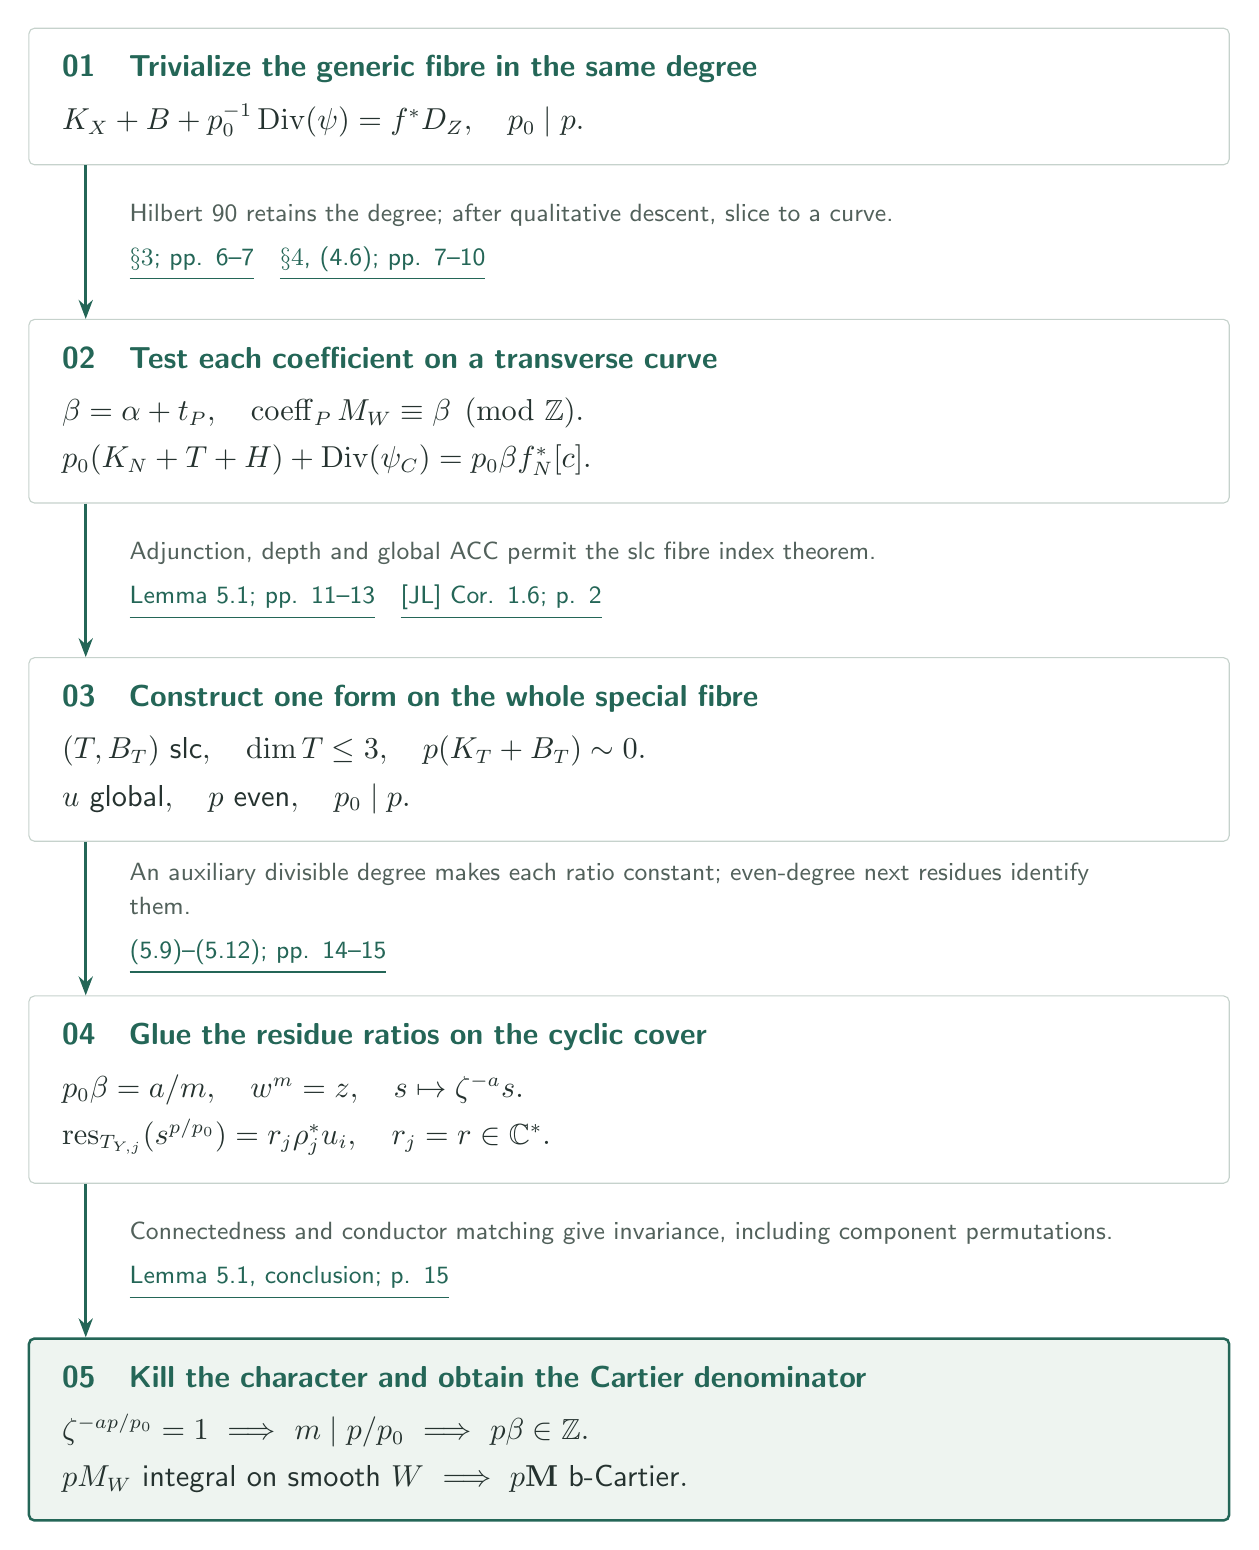
\begin{tikzpicture}
\node[card] (n0) {\heading{01}{一般ファイバーを同じ次数で自明化}{Trivialize the generic fibre in the same degree}$K_X+B+p_0^{-1}\operatorname{Div}(\psi)=f^*D_Z,\quad p_0\mid p.$};
\node[card,below=1.95cm of n0] (n1) {\heading{02}{各素因子の分母を曲線で測る}{Test each coefficient on a transverse curve}$\beta=\alpha+t_P,\quad \operatorname{coeff}_P M_W\equiv\beta\pmod{\mathbb Z}.$\\[3pt] $p_0(K_N+T+H)+\operatorname{Div}(\psi_C)=p_0\beta f_N^*[c].$};
\flow{n0}{n1}{\Tx{Hilbert 90で次数を保ち、定性的moduli降下の後に曲線へ切断。}{Hilbert 90 retains the degree; after qualitative descent, slice to a curve.}\\[4pt]\Cite{https://github.com/openai/math/blob/adc7f1241b42e322a6451854ab7e4b4c146bf78a/preprints/Relative-denominators-and-effective-systems-for-log-Calabi-Yau-fibrations-September-27-2026/paper.pdf}{$\S3$; pp. 6--7}\quad \Cite{https://github.com/openai/math/blob/adc7f1241b42e322a6451854ab7e4b4c146bf78a/preprints/Relative-denominators-and-effective-systems-for-log-Calabi-Yau-fibrations-September-27-2026/paper.pdf}{$\S4$, (4.6); pp. 7--10}}
\node[card,below=1.95cm of n1] (n2) {\heading{03}{特殊ファイバー全体に一つの形式を作る}{Construct one form on the whole special fibre}$(T,B_T)\text{ slc},\quad\dim T\le3,\quad p(K_T+B_T)\sim0.$\\[3pt] $u\text{ global},\quad p\text{ even},\quad p_0\mid p.$};
\flow{n1}{n2}{\Tx{dlt随伴・深さ・global ACCでslcファイバーの指数定理を適用。}{Adjunction, depth and global ACC permit the slc fibre index theorem.}\\[4pt]\Cite{https://github.com/openai/math/blob/adc7f1241b42e322a6451854ab7e4b4c146bf78a/preprints/Relative-denominators-and-effective-systems-for-log-Calabi-Yau-fibrations-September-27-2026/paper.pdf}{Lemma 5.1; pp. 11--13}\quad \Cite{https://arxiv.org/pdf/2002.11928v1}{[JL] Cor. 1.6; p. 2}}
\node[card,below=1.95cm of n2] (n3) {\heading{04}{巡回被覆上で留数の比をつなぐ}{Glue the residue ratios on the cyclic cover}$p_0\beta=a/m,\quad w^m=z,\quad s\mapsto\zeta^{-a}s.$\\[3pt] $\operatorname{res}_{T_{Y,j}}(s^{p/p_0})=r_j\rho_j^*u_i,\quad r_j=r\in\mathbb C^*.$};
\flow{n2}{n3}{\Tx{補助可除次数で各比を定数にし、偶数次数の次の留数で同一化。}{An auxiliary divisible degree makes each ratio constant; even-degree next residues identify them.}\\[4pt]\Cite{https://github.com/openai/math/blob/adc7f1241b42e322a6451854ab7e4b4c146bf78a/preprints/Relative-denominators-and-effective-systems-for-log-Calabi-Yau-fibrations-September-27-2026/paper.pdf}{(5.9)--(5.12); pp. 14--15}}
\node[result,below=1.95cm of n3] (n4) {\heading{05}{指標を消し、Cartier分母を得る}{Kill the character and obtain the Cartier denominator}$\zeta^{-ap/p_0}=1\ \Longrightarrow\ m\mid p/p_0\ \Longrightarrow\ p\beta\in\mathbb Z.$\\[3pt] $pM_W\text{ integral on smooth }W\ \Longrightarrow\ p\mathbf M\text{ b-Cartier}.$};
\flow{n3}{n4}{\Tx{連結性とconductorの整合性により、成分置換も含めて不変。}{Connectedness and conductor matching give invariance, including component permutations.}\\[4pt]\Cite{https://github.com/openai/math/blob/adc7f1241b42e322a6451854ab7e4b4c146bf78a/preprints/Relative-denominators-and-effective-systems-for-log-Calabi-Yau-fibrations-September-27-2026/paper.pdf}{Lemma 5.1, conclusion; p. 15}}
\end{tikzpicture}

\end{document}
